This document provides a brief description of the various structured meshes that are distributed with the library. Most of these meshes were developed for specific example codes but we expect them to be useful in other problems too. Many of the meshes exist in many different variants, usually constructed by multiple inheritance. When meshes are relatively trivial variations of each other, e.\+g. a basic mesh and its refineable equivalent, we only list the mesh once. The detailed documentation for the mesh (obtained by following the link) contains the full inheritance diagram, showing the mesh\textquotesingle{}s own base classes and any meshes that are derived from it. For each mesh, we provide a link to a fully-\/documented example problem that illustrates its use.

We stress that the {\bfseries key feature of any given mesh} is {\bfseries its topology}, rather than the specific shape for which it was originally developed. For instance, {\ttfamily oomph-\/lib} does not provide a mesh for the discretisation of an annular domain with quadrilateral elements. However, such a mesh is trivial to construct by deriving it from, e.\+g., the {\ttfamily Simple\+Rectangular\+Quad\+Mesh} (a mesh that discretises a rectangular domain), and then adjusting its nodal positions. Consult the example in the \href{../../../quick_guide/html/index.html#distorted_mesh}{\tt (Not-\/\+So-\/)Quick-\/\+Guide} for details.



 

\hypertarget{index_conventions}{}\section{Reminder\+: General conventions to facilitate the re-\/use of meshes}\label{index_conventions}
Since mesh generation tends to be most tedious part of any numerical simulation, {\ttfamily oomph-\/lib\textquotesingle{}s} overall data structure, described in detail \href{../../../the_data_structure/html/index.html}{\tt elsewhere, } aims to facilitate the re-\/use of meshes in many different applications. For this purpose most specific {\ttfamily Finite\+Elements} in {\ttfamily oomph-\/lib} are derived by multiple inheritance, combining a \char`\"{}geometric\char`\"{} {\ttfamily Finite\+Element} (e.\+g. a line/quadrilateral/brick-\/shaped element from the {\ttfamily Q\+Element$<$\+D\+I\+M,\+N\+N\+O\+D\+E\+\_\+1\+D$>$} family) with an equations class (such as {\ttfamily Poisson\+Equations$<$\+D\+I\+M$>$}) that implements the weak form of a specific P\+DE. For instance, {\ttfamily oomph-\/lib\textquotesingle{}s} quadrilateral nine-\/node Poisson element, {\ttfamily Q\+Poisson\+Element$<$2,3$>$}, is derived from the {\ttfamily Poisson\+Equations$<$2$>$} equations class and the {\ttfamily Q\+Element$<$2,3$>$} geometric {\ttfamily Finite\+Element}.

The mesh generation process is mainly concerned with the geometric properties of the mesh\textquotesingle{}s constituent {\ttfamily Finite\+Elements} (their topology, number of nodes, etc.) which are defined by the geometric {\ttfamily Finite\+Element}. This makes it possible to use a mesh that was originally developed for the solution of a Poisson equation with a {\ttfamily Q\+Poisson\+Element$<$2,\+N\+N\+O\+D\+E\+\_\+1\+D$>$}, say, for the solution of an advection-\/diffusion problem with a {\ttfamily Q\+Advction\+Diffusion\+Element$<$2,\+N\+N\+O\+D\+E\+\_\+1\+D$>$} since both elements are derived from the same geometric {\ttfamily Finite\+Element}. Only two aspects of the mesh generation process require information that is not provided by the geometric {\ttfamily Finite\+Element\+:} 
\begin{DoxyItemize}
\item {\bfseries The number of values to be stored at the various nodes in the mesh\+:} For instance, if a mesh that is designed for quadrilateral elements from the {\ttfamily Q\+Element$<$2,\+N\+N\+O\+D\+E\+\_\+1\+D$>$} family of geometric elements is used to solve a (scalar) Poisson equation with nine-\/noded elements, each {\ttfamily Node} has to store a single value. However, if the same mesh is used for the solution of the 2D Navier-\/\+Stokes equations with a nine-\/node quadrilateral elements of type {\ttfamily Q\+Taylor\+Hood\+Element$<$2$>$}, nodes located at the elements\textquotesingle{} four vertices have to store three values (two velocity components and one pressure) whereas nodes located at the elements\textquotesingle{} interior and on their edges only have to store two values (the two velocity components). ~\newline
~\newline

\item {\bfseries The number of \char`\"{}history values\char`\"{} required by the timestepping procedure (if any)\+:} For instance, if the mesh is used for the solution of a Poisson problem, no \char`\"{}history\char`\"{} values are required. If the same mesh is used for the solution of an unsteady heat problem, the number of history values required is determined by the {\ttfamily Time\+Stepper} used to approximate the time-\/derivative of the nodal values.
\end{DoxyItemize}The meshes used in our example codes (and all the meshes listed below) have a common structure that allows the required information to be become available to the mesh constructor\+:
\begin{DoxyEnumerate}
\item All meshes are templated by the element type, {\ttfamily E\+L\+E\+M\+E\+NT}.~\newline
~\newline

\item The final argument of all mesh constructors is a pointer to a {\ttfamily Time\+Stepper}. We provide a default for this argument -- a pointer to the {\ttfamily Steady$<$0$>$} timestepper, defined (as static member data) in the {\ttfamily Mesh} base class.
\end{DoxyEnumerate}The availability of the template parameter allows the mesh generator to build elements of the required type. {\ttfamily Nodes} are generally built by the {\ttfamily Finite\+Element\+::construct\+\_\+node}(...) function whose arguments are the {\ttfamily Node\textquotesingle{}s} local node number within the current element, and a pointer to the timestepper. These arguments provide all the information that is required to build {\ttfamily Nodes} with the right number of values (as required by the element) and history values (as required by the {\ttfamily Time\+Stepper}). When the function {\ttfamily Finite\+Element\+::construct\+\_\+node}(...) is called, it creates the new {\ttfamily Node}, stores a pointer to the newly created {\ttfamily Node} in the {\ttfamily Finite\+Element\textquotesingle{}s} own lookup scheme, and returns that pointer. This allows the pointer to the newly created {\ttfamily Node} to be stored in the {\ttfamily Mesh\textquotesingle{}s} own lookup scheme for its constituent {\ttfamily Nodes}. The \href{../../../quick_guide/html/index.html#mesh}{\tt (Not-\/\+So-\/)Quick-\/\+Guide} contains a section that explains how to write simple meshes. 

 

\hypertarget{index_faq}{}\section{Mesh F\+AQ}\label{index_faq}
When using a mesh that was originally developed for a different application, it is sometimes necessary establish the node/element/boundary numbering scheme employed by the mesh writer. While we generally assume that the mesh writer will have carefully documented his/her code, here is what to do if he/she hasn\textquotesingle{}t\+: ~\newline
~\newline

\begin{DoxyItemize}
\item {\bfseries How do I find out how the elements are numbered?} ~\newline
~\newline
 The function {\ttfamily Mesh\+::output}(...) outputs the elements in the order in which they are stored internally. If you prefer a different element numbering scheme you can re-\/number the elements; see e.\+g. the member function {\ttfamily element\+\_\+reorder()} in the \href{classoomph_1_1RectangularQuadMesh.html}{\tt {\bfseries  Rectangular\+Quad\+Mesh}} class. ~\newline
~\newline

\item {\bfseries How do I find out how the nodes are numbered?} ~\newline
~\newline
 The function {\ttfamily Mesh\+::node\+\_\+pt(j)} provides pointer-\/based access to the {\ttfamily j} -\/ th {\ttfamily Node} in the mesh. To plot a node\textquotesingle{}s position, you can determine its coordinates from the {\ttfamily Node\+::x}(...) function. ~\newline
~\newline

\item {\bfseries How do I find out how the mesh boundaries are numbered?} ~\newline
~\newline
 The function {\ttfamily Mesh\+::output\+\_\+boundaries}(...) outputs the nodes located on the mesh boundaries in a \href{http://www.tecplot.com}{\tt tecplot}-\/able format. Nodes that are located on separate mesh boundaries are contained in separate \href{http://www.tecplot.com}{\tt tecplot} zones. ~\newline
~\newline

\end{DoxyItemize}With this information it should be straightforward to use any of the meshes listed below in one of your own problems. The example code listed next to each mesh illustrates its use in an actual driver code. If you develop a new mesh, let us know! If it is written according to {\ttfamily oomph-\/lib\textquotesingle{}s} \href{../../../coding_conventions/html/index.html}{\tt coding standards}, we\textquotesingle{}ll be delighted to include it into the library.



 

\hypertarget{index_mesh_list}{}\section{Mesh list}\label{index_mesh_list}
\begin{center} \tabulinesep=1mm
\begin{longtabu} spread 0pt [c]{*{2}{|X[-1]}|}
\hline
{\bfseries Mesh}  &{\bfseries Representative Mesh plot}   \\\cline{1-2}
\href{classoomph_1_1OneDMesh.html}{\tt {\bfseries  One\+D\+Mesh$<$\+E\+L\+E\+M\+E\+N\+T$>$ }} ~\newline
~\newline

\begin{DoxyItemize}
\item This mesh can be used with all {\ttfamily Finite\+Elements} that are derived from the geometric finite element {\ttfamily Q\+Element$<$1,\+N\+N\+O\+D\+E\+\_\+1\+D$>$}.
\item This mesh forms the basis for numerous derived meshes.
\item A refineable version of this mesh exists.
\end{DoxyItemize}{\bfseries Example driver code\+:} ~\newline

\begin{DoxyItemize}
\item This mesh is used in the driver code for \href{../../../poisson/one_d_poisson/html/index.html}{\tt the solution of the 1D Poisson equation. }
\end{DoxyItemize}& 
\begin{DoxyImageNoCaption}
  \mbox{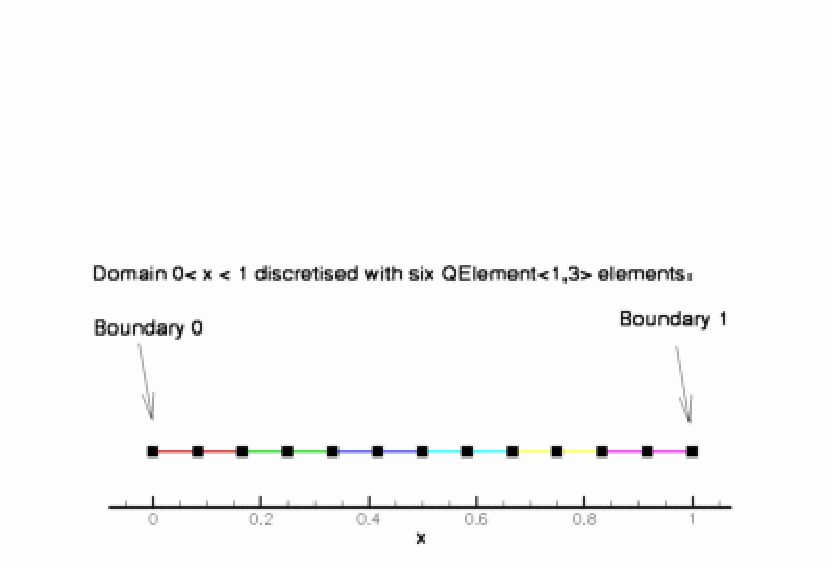
\includegraphics[width=0.75\textwidth]{one_d_mesh}}
\end{DoxyImageNoCaption}
   \\\cline{1-2}
\href{classoomph_1_1SimpleRectangularQuadMesh.html}{\tt {\bfseries  Simple\+Rectangular\+Quad\+Mesh$<$\+E\+L\+E\+M\+E\+N\+T$>$ }} ~\newline
~\newline

\begin{DoxyItemize}
\item This mesh can be used with all {\ttfamily Finite\+Elements} that are derived from the geometric finite element {\ttfamily Q\+Element$<$2,\+N\+N\+O\+D\+E\+\_\+1\+D$>$}.
\item This mesh forms the basis for numerous derived meshes.
\end{DoxyItemize}{\bfseries Example driver code\+:} ~\newline

\begin{DoxyItemize}
\item This mesh is used in the driver code for \href{../../../poisson/two_d_poisson/html/index.html}{\tt the solution of the 2D Poisson equation. }
\end{DoxyItemize}& 
\begin{DoxyImageNoCaption}
  \mbox{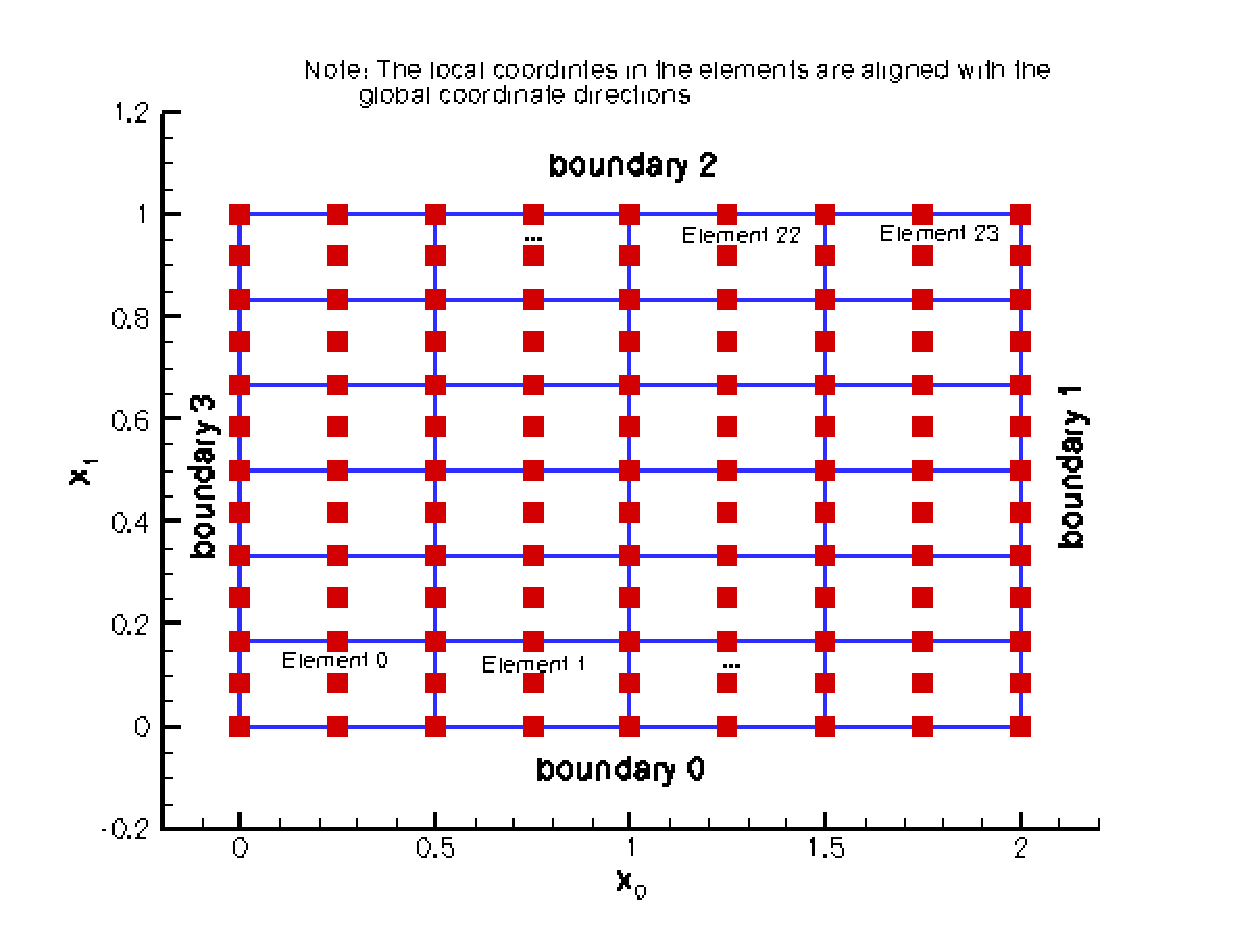
\includegraphics[width=0.75\textwidth]{simple_rectangular_quadmesh}}
\end{DoxyImageNoCaption}
   \\\cline{1-2}
\href{classoomph_1_1RectangularQuadMesh.html}{\tt {\bfseries  Rectangular\+Quad\+Mesh$<$\+E\+L\+E\+M\+E\+N\+T$>$ }} ~\newline
~\newline

\begin{DoxyItemize}
\item This is a slightly more sophisticated version of the {\ttfamily Simple\+Rectangular\+Quad\+Mesh} discussed above; it allows for non-\/uniform spacing of the nodes, and periodicity in the x and y-\/directions.
\item This mesh can be used with all {\ttfamily Finite\+Elements} that are derived from the geometric finite element {\ttfamily Q\+Element$<$2,\+N\+N\+O\+D\+E\+\_\+1\+D$>$}.
\item This mesh forms the basis for numerous derived meshes.
\item A refineable version of this mesh exists.
\end{DoxyItemize}{\bfseries Example driver code\+:} ~\newline

\begin{DoxyItemize}
\item The refineable variant of this mesh is used in the driver code for \href{../../../advection_diffusion/two_d_adv_diff_adapt/html/index.html}{\tt the solution of the 2D Advection Diffusion equation. }
\end{DoxyItemize}& 
\begin{DoxyImageNoCaption}
  \mbox{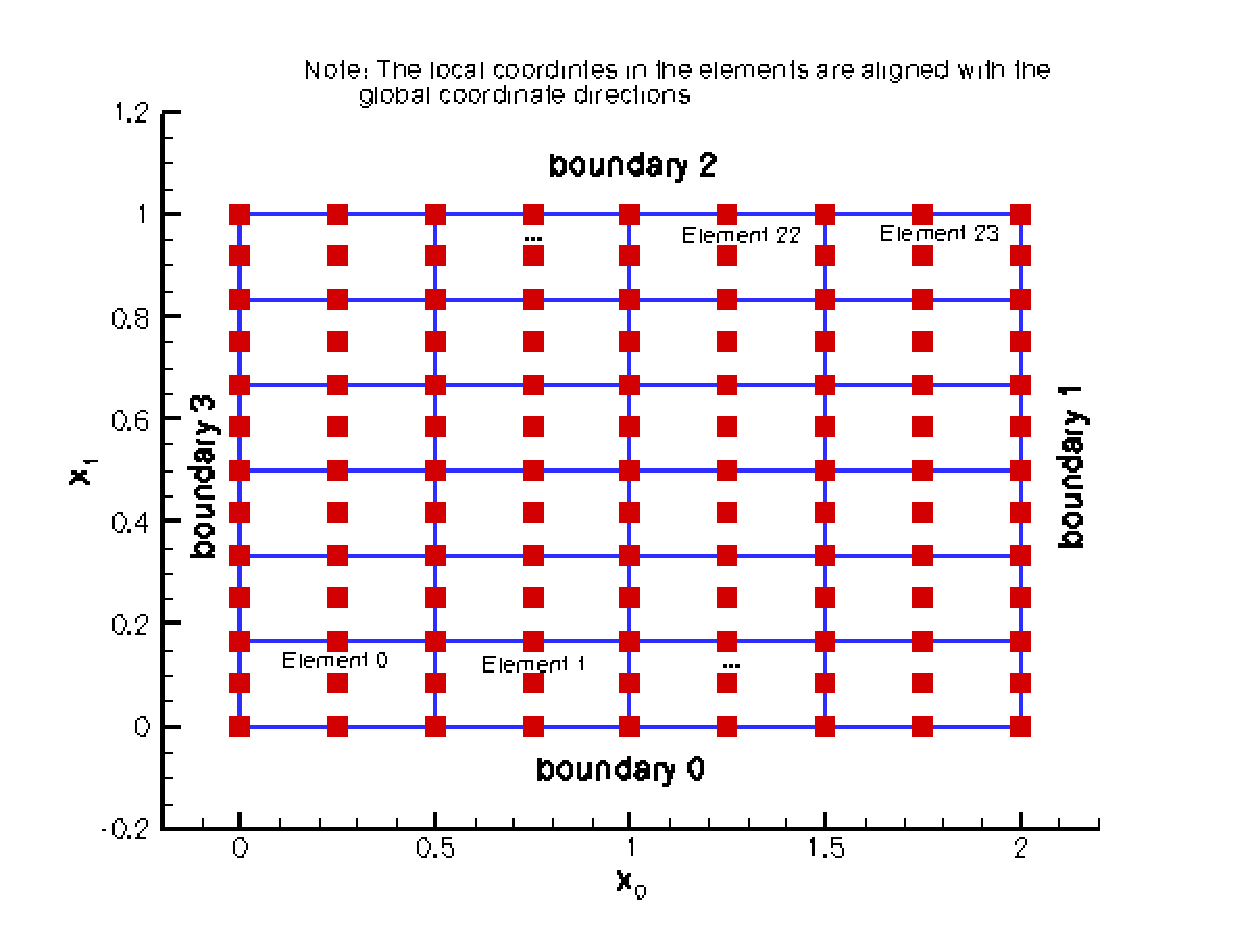
\includegraphics[width=0.75\textwidth]{simple_rectangular_quadmesh}}
\end{DoxyImageNoCaption}
   \\\cline{1-2}
\href{classoomph_1_1TwoDAnnularMesh.html}{\tt {\bfseries  Two\+D\+Annular\+Mesh$<$\+E\+L\+E\+M\+E\+N\+T$>$ }} ~\newline
~\newline

\begin{DoxyItemize}
\item This is a \char`\"{}wrapped around\char`\"{} version of {\ttfamily Rectangular\+Quad\+Mesh} discussed above. It can either be used as a complete annulus (in which case periodicity is enforced) or a gap can appear in the annulus.
\item This mesh can be used with all {\ttfamily Finite\+Elements} that are derived from the geometric finite element {\ttfamily Q\+Element$<$2,\+N\+N\+O\+D\+E\+\_\+1\+D$>$}.
\item A refineable version of this mesh exists.
\end{DoxyItemize}{\bfseries Example driver code\+:} ~\newline

\begin{DoxyItemize}
\item This mesh is used in the driver code for \href{../../../helmholtz/scattering/html/index.html}{\tt the 2D Helmholtz equation}and the \href{../../../time_harmonic_linear_elasticity/elastic_annulus/html/index.html}{\tt time-\/harmonic linear elasticity equations}. 
\end{DoxyItemize}& 
\begin{DoxyImageNoCaption}
  \mbox{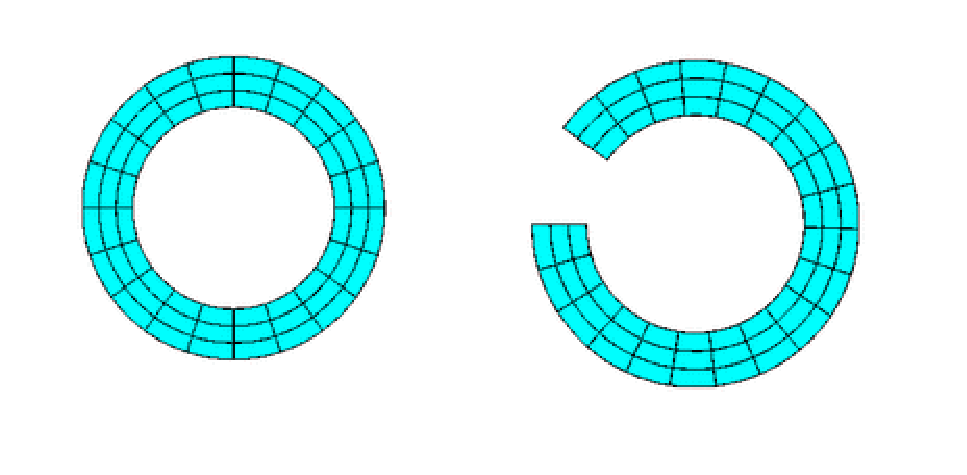
\includegraphics[width=0.75\textwidth]{annular_meshes}}
\end{DoxyImageNoCaption}
   \\\cline{1-2}
\label{_channel_with_leaflet}%
 \href{classoomph_1_1ChannelWithLeafletMesh.html}{\tt {\bfseries  Channel\+With\+Leaflet\+Mesh$<$\+E\+L\+E\+M\+E\+N\+T$>$ }} ~\newline
~\newline

\begin{DoxyItemize}
\item Mesh for the simulation of flow in a 2D channel that is partially occluded by a moving leaflet.
\item Leaflet must be represented by a {\ttfamily Geom\+Object} 
\item Nodes along the leaflet are duplicated to allow for a pressure jump across the leaflet even for discretisations that impose continuous pressure distributions across element boundaries.
\item This mesh can be used with all {\ttfamily Finite\+Elements} that are derived from the geometric finite element {\ttfamily Q\+Element$<$2,\+N\+N\+O\+D\+E\+\_\+1\+D$>$}.
\item This mesh forms the basis for numerous derived meshes.
\item A refineable version of this mesh exists.
\end{DoxyItemize}{\bfseries Example driver code\+:} ~\newline

\begin{DoxyItemize}
\item The refineable variant of this mesh with an algebraic node update is used in the driver code for \href{../../../navier_stokes/channel_with_leaflet/html/index.html}{\tt the simulation of flow in a 2D channel that is partially occluded by a moving leaflet} and also in \href{../../../interaction/fsi_channel_with_leaflet/html/index.html}{\tt corresponding F\+SI problem. }
\end{DoxyItemize}& 
\begin{DoxyImageNoCaption}
  \mbox{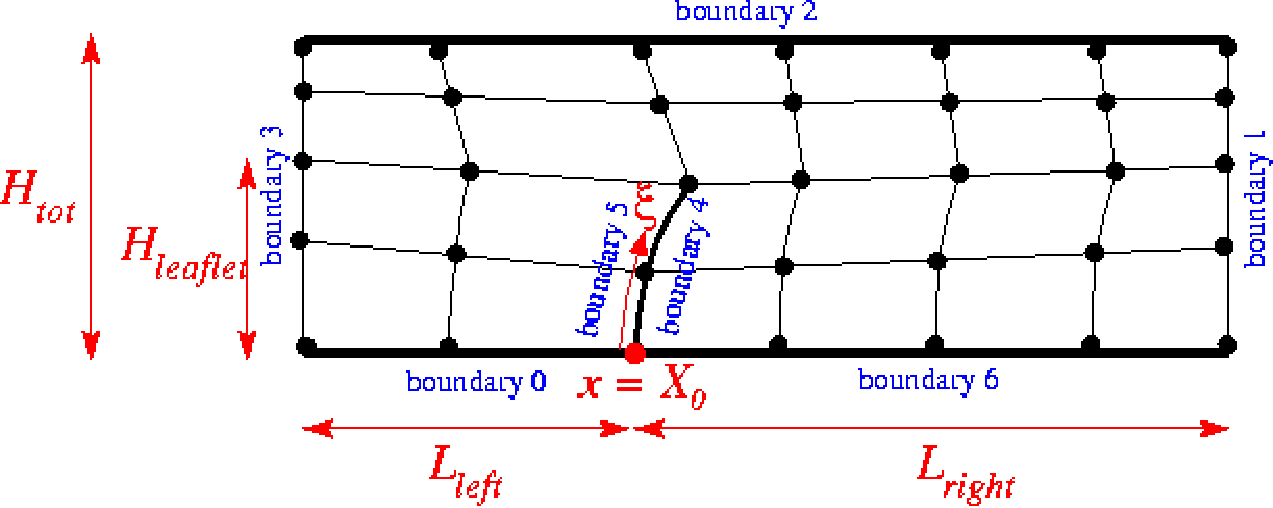
\includegraphics[width=0.75\textwidth]{channel_with_leaflet_mesh}}
\end{DoxyImageNoCaption}
   \\\cline{1-2}
\href{classoomph_1_1SimpleRectangularTriMesh.html}{\tt {\bfseries  Simple\+Rectangular\+Tri\+Mesh$<$\+E\+L\+E\+M\+E\+N\+T$>$ }} ~\newline
~\newline

\begin{DoxyItemize}
\item This is a simple structured mesh made of triangular elements.
\item This mesh can be used with all {\ttfamily Finite\+Elements} that are derived from the geometric finite element {\ttfamily T\+Element$<$2,\+N\+N\+O\+D\+E\+\_\+1\+D$>$}.
\end{DoxyItemize}{\bfseries Example driver code\+:} ~\newline

\begin{DoxyItemize}
\item This mesh is used in the self-\/test code \href{../../../../self_test/poisson/convergence_tests/t_convergence_2d.cc}{\tt {\ttfamily t\+\_\+convergence\+\_\+2d.\+cc} }
\end{DoxyItemize}& 
\begin{DoxyImageNoCaption}
  \mbox{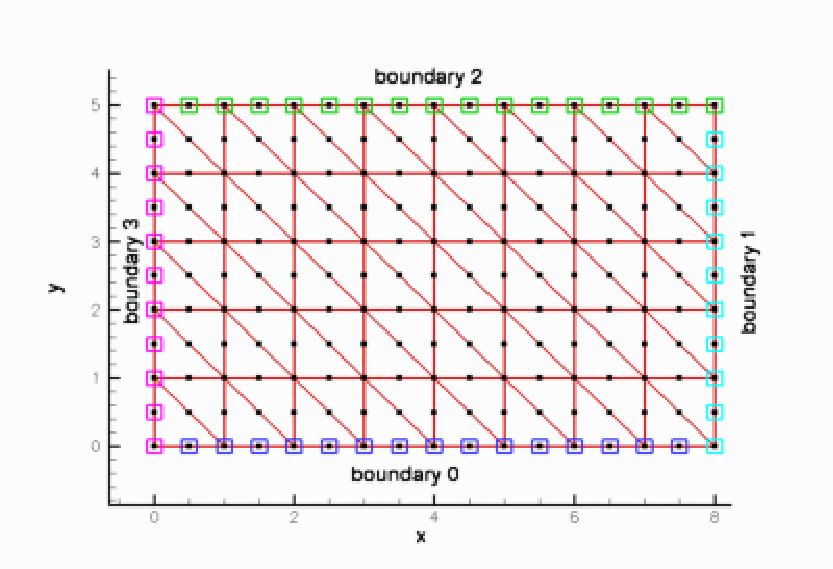
\includegraphics[width=0.75\textwidth]{simple_rectangular_trimesh}}
\end{DoxyImageNoCaption}
   \\\cline{1-2}
\href{classoomph_1_1FishMesh.html}{\tt {\bfseries  Fish\+Mesh$<$\+E\+L\+E\+M\+E\+N\+T$>$ }} ~\newline
~\newline

\begin{DoxyItemize}
\item This mesh can be used with all {\ttfamily Finite\+Elements} that are derived from the geometric finite element {\ttfamily Q\+Element$<$2,\+N\+N\+O\+D\+E\+\_\+1\+D$>$}.
\item This mesh forms the basis for numerous derived meshes.
\item The curvilinear boundaries are represented by a {\ttfamily Geom\+Object} and the mesh has a {\ttfamily Domain} representation, allowing a {\ttfamily Macro\+Element} -\/ based node update.
\item There is also a version of the mesh that performs the node update in response to changes in the domain boundary by an algebraic node update.
\item A refineable version of this mesh exists.
\end{DoxyItemize}{\bfseries Example driver code\+:} ~\newline

\begin{DoxyItemize}
\item The refineable variant of this mesh is used in the driver code for \href{../../../poisson/fish_poisson/html/index.html}{\tt the adaptive solution of the 2D Poisson equation in a fish-\/shaped domain. }
\end{DoxyItemize}& 
\begin{DoxyImageNoCaption}
  \mbox{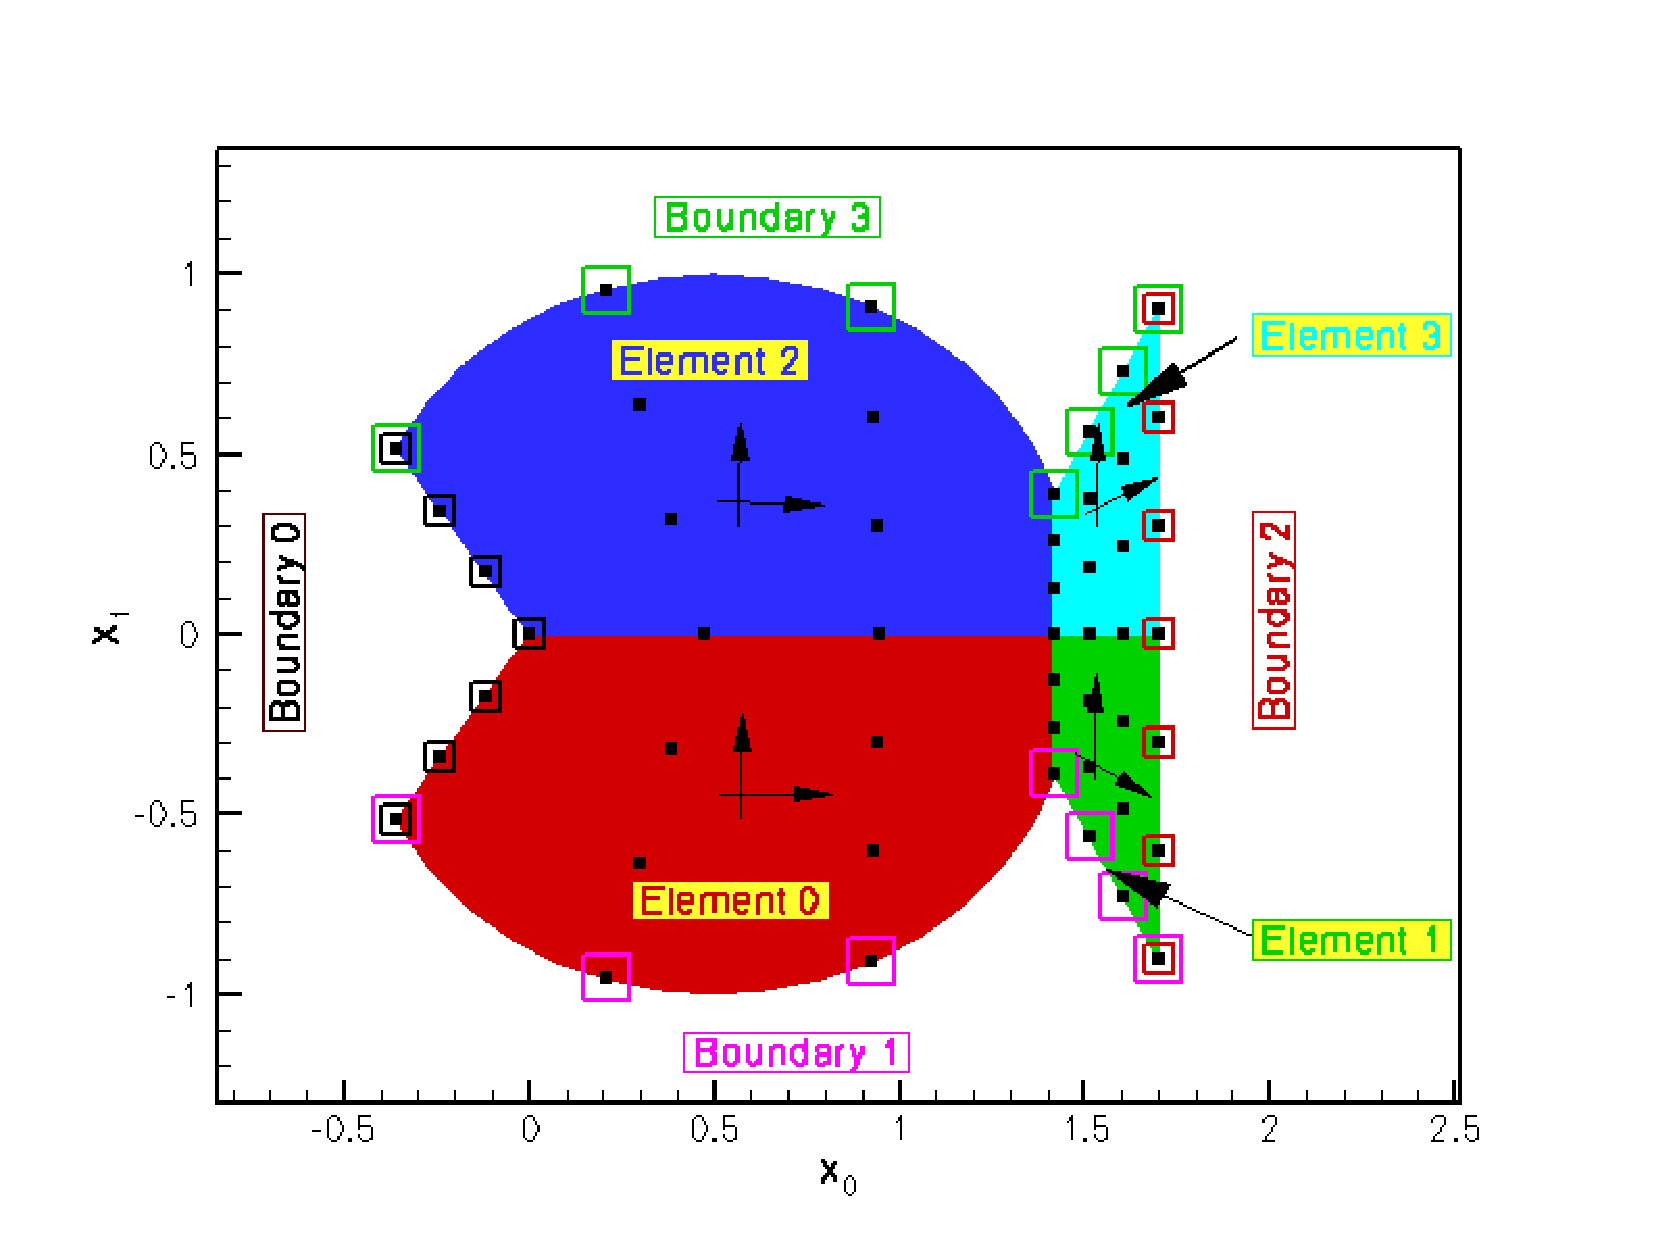
\includegraphics[width=0.75\textwidth]{fish_mesh}}
\end{DoxyImageNoCaption}
   \\\cline{1-2}
\label{_collapsible_channel}%
 \href{classoomph_1_1CollapsibleChannelMesh.html}{\tt {\bfseries  Collapsible\+Channel\+Mesh$<$\+E\+L\+E\+M\+E\+N\+T$>$ }} ~\newline
~\newline

\begin{DoxyItemize}
\item This mesh can be used with all {\ttfamily Finite\+Elements} that are derived from the geometric finite element {\ttfamily Q\+Element$<$2,\+N\+N\+O\+D\+E\+\_\+1\+D$>$}.
\item This mesh forms the basis for numerous derived meshes
\item The curvilinear boundary is represented by a {\ttfamily Geom\+Object} and the mesh has a {\ttfamily Domain} representation, allowing a {\ttfamily Macro\+Element} -\/ based node update.
\item There is also a version of the mesh that performs the node update in response to changes in the domain boundary by an algebraic node update.
\item A refineable version of this mesh exists.
\end{DoxyItemize}{\bfseries Example driver code\+:} ~\newline

\begin{DoxyItemize}
\item This mesh is used in the driver code for \href{../../../navier_stokes/collapsible_channel/html/index.html}{\tt the solution of the 2D unsteady Navier-\/\+Stokes equations in 2D channel with an oscillating wall. }
\end{DoxyItemize}& 
\begin{DoxyImageNoCaption}
  \mbox{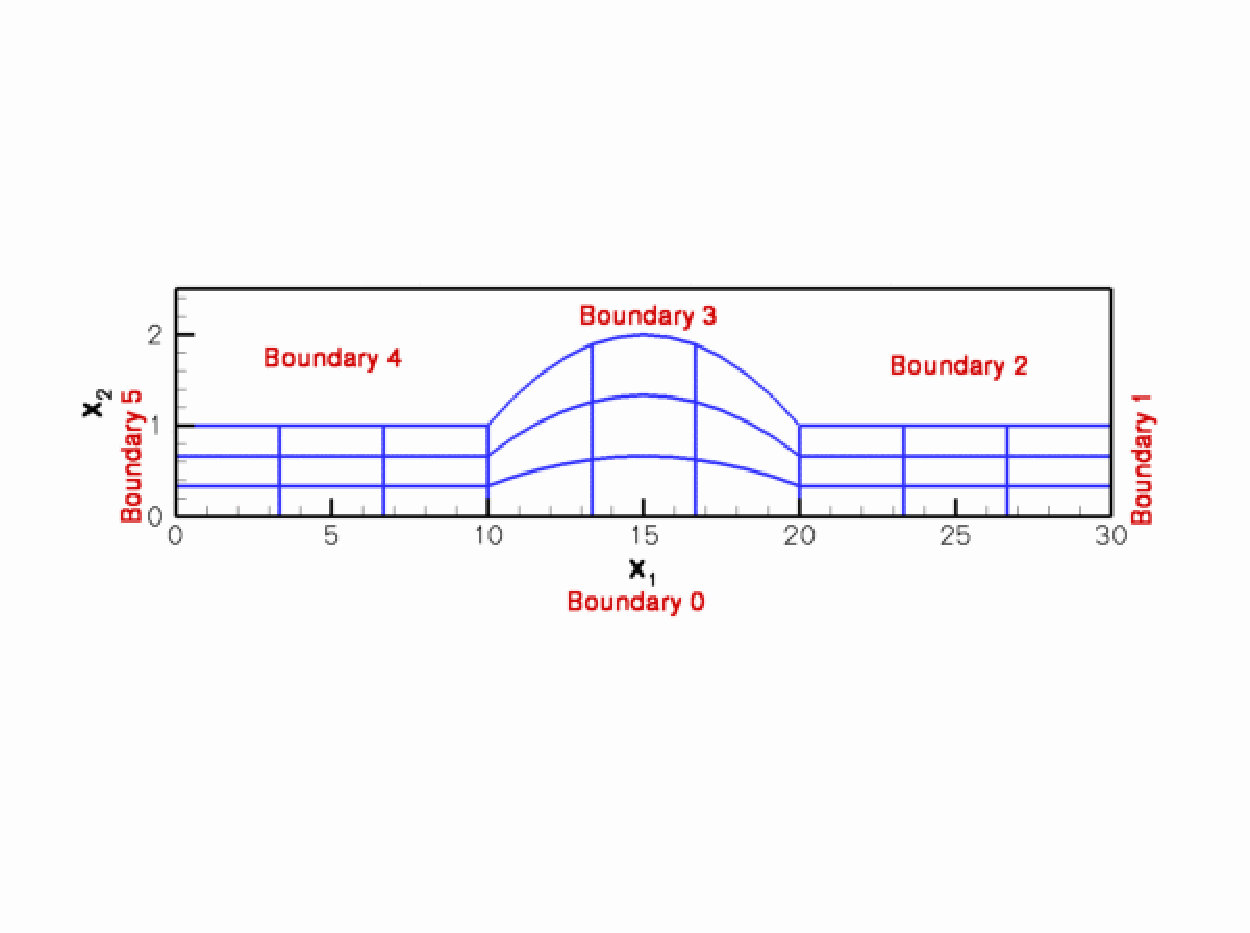
\includegraphics[width=0.75\textwidth]{collapsible_channel_mesh}}
\end{DoxyImageNoCaption}
   \\\cline{1-2}
\href{classoomph_1_1CylinderWithFlagMesh.html}{\tt {\bfseries  Cylinder\+With\+Flag\+Mesh$<$\+E\+L\+E\+M\+E\+N\+T$>$ }} ~\newline
~\newline

\begin{DoxyItemize}
\item This {\ttfamily Mesh} was mainly developed for the solution of Turek \& Hron\textquotesingle{}s F\+SI benchmark problems. The curvilinear boundaries of the cylinder and the \char`\"{}flag\char`\"{} are represented by {\ttfamily Geom\+Objects}.
\item A refineable version of the mesh exists.
\item The node-\/update in response to changes in the shape of the \char`\"{}flag\char`\"{} can be performed by a version based on an {\ttfamily Algebraic\+Mesh} or using a {\ttfamily Domain/\+Macro\+Element} -\/ based node update.
\item The bulk elements have to be derived from the geometric finite element {\ttfamily Q\+Element$<$2,\+N\+N\+O\+D\+E\+\_\+1\+D$>$}.
\end{DoxyItemize}{\bfseries Example driver code\+:} ~\newline

\begin{DoxyItemize}
\item This mesh is used in the driver code for \href{../../../interaction/turek_flag/html/index.html}{\tt Turek \& Hron\textquotesingle{}s F\+SI benchmark problems } and their \href{../../../navier_stokes/turek_flag_non_fsi/html/index.html}{\tt non-\/\+F\+SI equivalents.}
\end{DoxyItemize}& 
\begin{DoxyImageNoCaption}
  \mbox{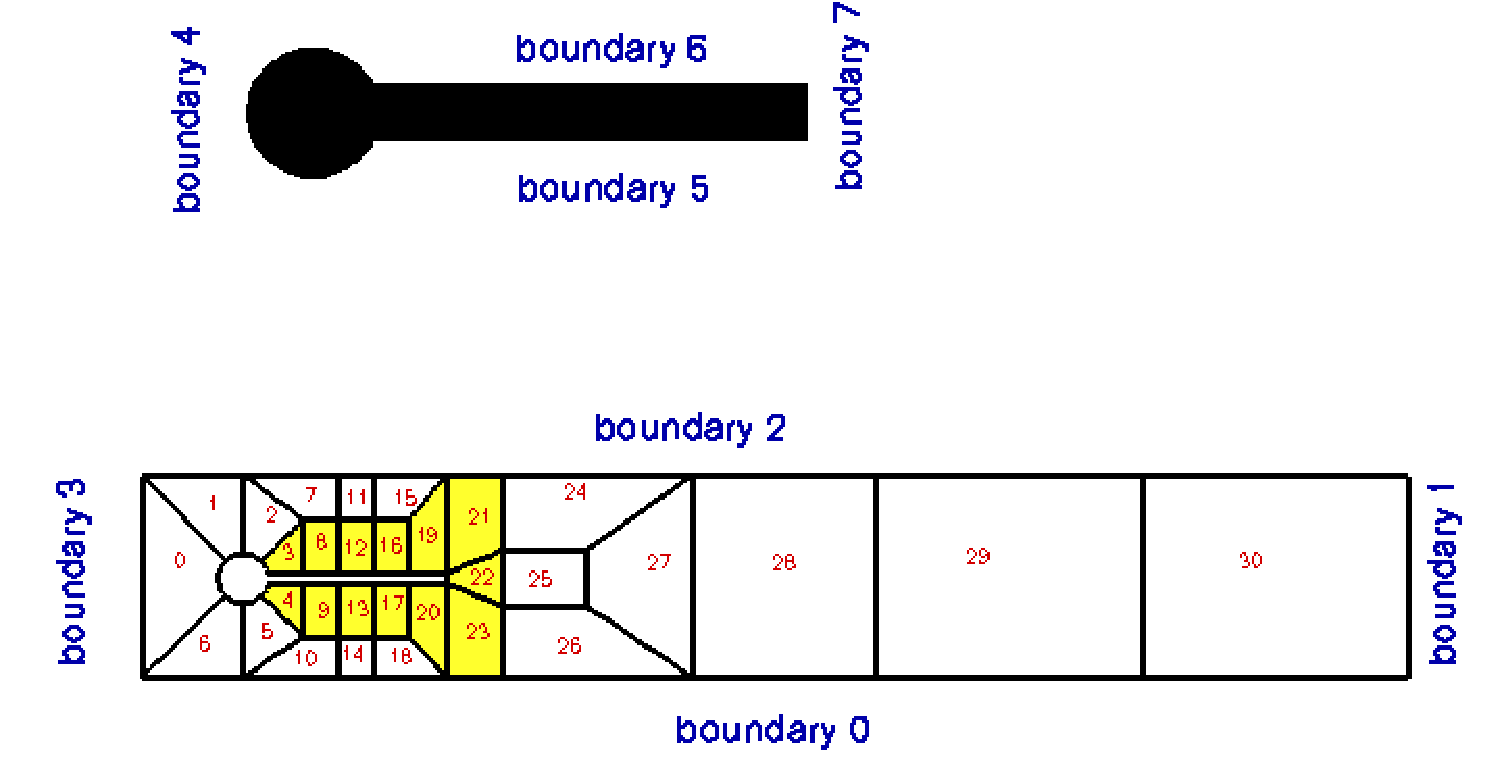
\includegraphics[width=0.75\textwidth]{cylinder_with_flag_mesh}}
\end{DoxyImageNoCaption}
   \\\cline{1-2}
\href{classoomph_1_1BrethertonSpineMesh.html}{\tt {\bfseries  Bretherton\+Spine\+Mesh$<$\+E\+L\+E\+M\+E\+N\+T$>$ }} ~\newline
~\newline

\begin{DoxyItemize}
\item This {\ttfamily Spine\+Mesh} was mainly developed for the simulation of the Bretherton problem but it can, of course, also be used in other problems. The mesh topology would be suitable for the simulation of flows in a bifurcating channel, say.
\item The bulk elements have to be derived from the geometric finite element {\ttfamily Q\+Element$<$2,\+N\+N\+O\+D\+E\+\_\+1\+D$>$}.
\end{DoxyItemize}{\bfseries Example driver code\+:} ~\newline

\begin{DoxyItemize}
\item This mesh is used in the driver code for \href{../../../navier_stokes/bretherton/html/index.html}{\tt the simulation of the Bretherton problem. }
\end{DoxyItemize}& 
\begin{DoxyImageNoCaption}
  \mbox{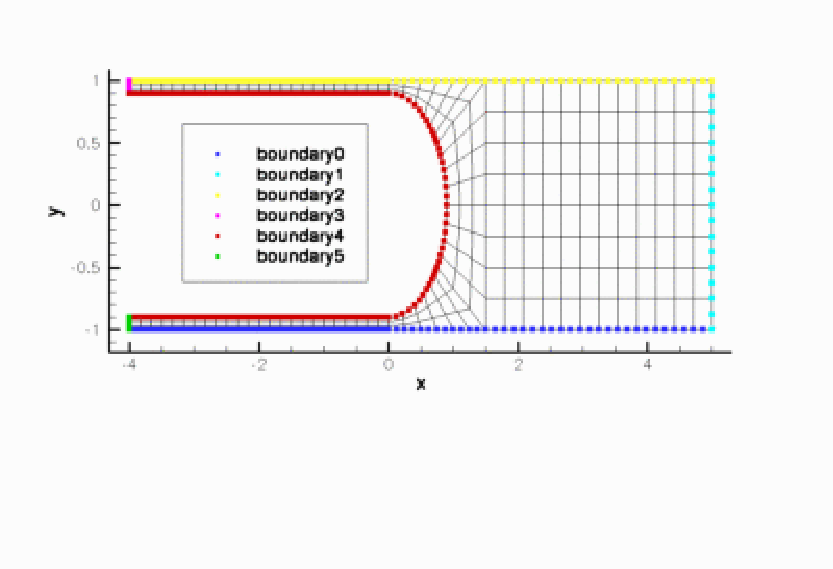
\includegraphics[width=0.75\textwidth]{bretherton_spine_mesh}}
\end{DoxyImageNoCaption}
   \\\cline{1-2}
\href{classoomph_1_1QuarterCircleSectorMesh.html}{\tt {\bfseries  Quarter\+Circle\+Sector\+Mesh$<$\+E\+L\+E\+M\+E\+N\+T$>$ }} ~\newline
~\newline

\begin{DoxyItemize}
\item This mesh can be used with all {\ttfamily Finite\+Elements} that are derived from the geometric finite element {\ttfamily Q\+Element$<$2,\+N\+N\+O\+D\+E\+\_\+1\+D$>$}.
\item This mesh forms the basis for numerous derived meshes
\item The curvilinear boundary is represented by a {\ttfamily Geom\+Object} and the mesh has a {\ttfamily Domain} representation, allowing a {\ttfamily Macro\+Element} -\/ based node update.
\item There is also a version of the mesh that performs the node update in response to changes in the domain boundary by an algebraic node update.
\item A refineable version of this mesh exists.
\end{DoxyItemize}{\bfseries Example driver code\+:} ~\newline

\begin{DoxyItemize}
\item The refineable version of this mesh is used in the driver code for \href{../../../navier_stokes/osc_ellipse/html/index.html}{\tt the simulation of flow inside a oscillating ellipse. }
\end{DoxyItemize}& 
\begin{DoxyImageNoCaption}
  \mbox{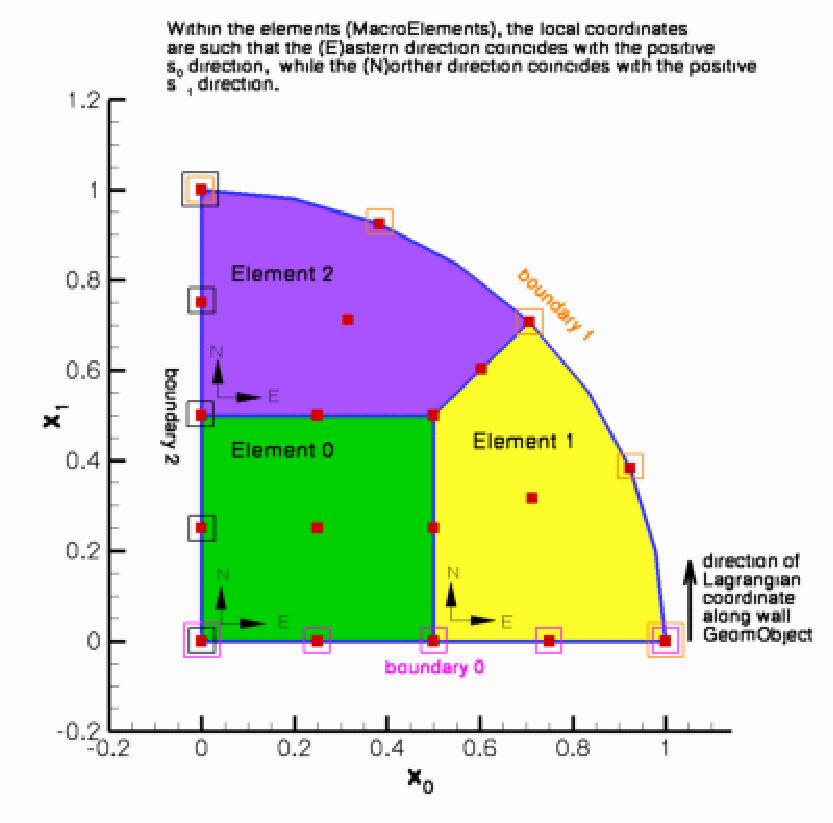
\includegraphics[width=0.75\textwidth]{quarter_circle_sector_mesh}}
\end{DoxyImageNoCaption}
   \\\cline{1-2}
\href{classoomph_1_1SimpleCubicMesh.html}{\tt {\bfseries  Simple\+Cubic\+Mesh$<$\+E\+L\+E\+M\+E\+N\+T$>$ }} ~\newline
~\newline

\begin{DoxyItemize}
\item This mesh can be used with all {\ttfamily Finite\+Elements} that are derived from the geometric finite element {\ttfamily Q\+Element$<$3,\+N\+N\+O\+D\+E\+\_\+1\+D$>$}.
\item A refineable version of this mesh exists.
\end{DoxyItemize}{\bfseries Example driver code\+:} ~\newline

\begin{DoxyItemize}
\item This mesh is used in the self-\/test code \href{../../../../self_test/poisson/convergence_tests/q_convergence_3d.cc}{\tt {\ttfamily q\+\_\+convergence\+\_\+3d.\+cc} }
\end{DoxyItemize}& 
\begin{DoxyImageNoCaption}
  \mbox{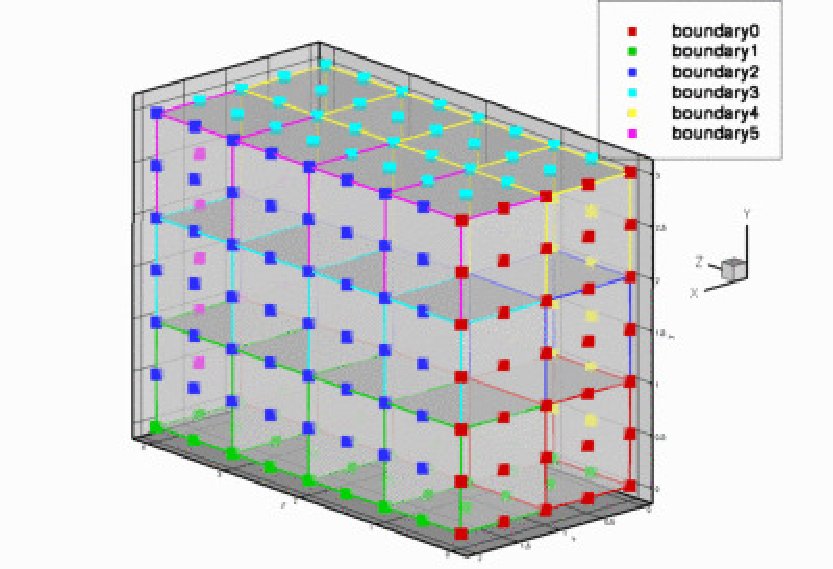
\includegraphics[width=0.75\textwidth]{simple_cubic_mesh}}
\end{DoxyImageNoCaption}
   \\\cline{1-2}
\href{classoomph_1_1SimpleCubicTetMesh.html}{\tt {\bfseries  Simple\+Cubic\+Tet\+Mesh$<$\+E\+L\+E\+M\+E\+N\+T$>$ }} ~\newline
~\newline

\begin{DoxyItemize}
\item This is a simple structured mesh for tet elements.
\item This mesh can be used with all {\ttfamily Finite\+Elements} that are derived from the geometric finite element {\ttfamily T\+Element$<$3,\+N\+N\+O\+D\+E\+\_\+1\+D$>$}.
\end{DoxyItemize}{\bfseries Example driver code\+:} ~\newline

\begin{DoxyItemize}
\item This mesh is used in the self-\/test code \href{../../../../self_test/poisson/convergence_tests/t_convergence_3d.cc}{\tt {\ttfamily t\+\_\+convergence\+\_\+3d.\+cc} }
\end{DoxyItemize}& 
\begin{DoxyImageNoCaption}
  \mbox{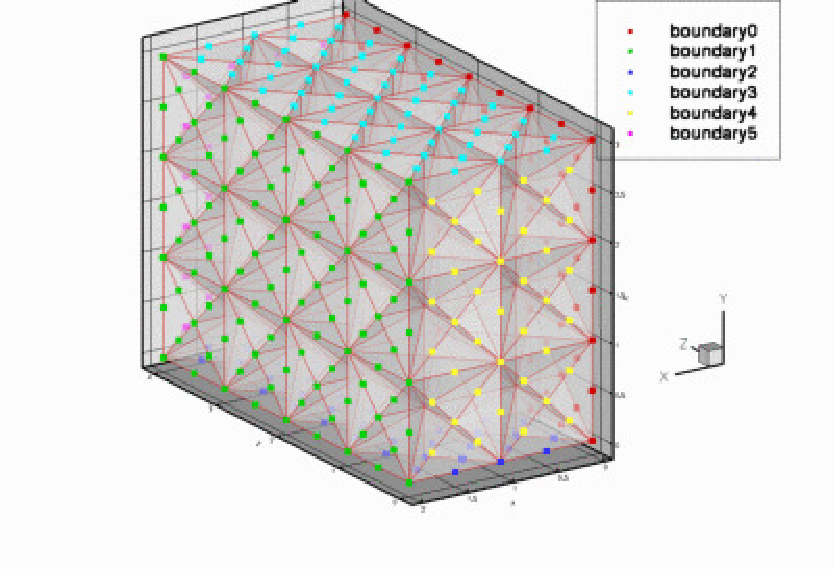
\includegraphics[width=0.75\textwidth]{simple_cubic_tetmesh}}
\end{DoxyImageNoCaption}
   \\\cline{1-2}
\href{classoomph_1_1QuarterTubeMesh.html}{\tt {\bfseries  Quarter\+Tube\+Mesh$<$\+E\+L\+E\+M\+E\+N\+T$>$ }} ~\newline
~\newline

\begin{DoxyItemize}
\item This mesh can be used with all {\ttfamily Finite\+Elements} that are derived from the geometric finite element {\ttfamily Q\+Element$<$3,\+N\+N\+O\+D\+E\+\_\+1\+D$>$}.
\item This mesh forms the basis for numerous derived meshes
\item The curvilinear boundary is represented by a {\ttfamily Geom\+Object} and the mesh has a {\ttfamily Domain} representation, allowing a {\ttfamily Macro\+Element} -\/ based node update.
\item There is also a version of the mesh that performs the node update in response to changes in the domain boundary by an algebraic node update.
\item A refineable version of this mesh exists.
\end{DoxyItemize}{\bfseries Example driver code\+:} ~\newline

\begin{DoxyItemize}
\item The refineable version of this mesh is used in the driver code for \href{../../../navier_stokes/three_d_entry_flow/html/index.html}{\tt the simulation of 3D entry flow into a cylindrical tube. }
\end{DoxyItemize}& 
\begin{DoxyImageNoCaption}
  \mbox{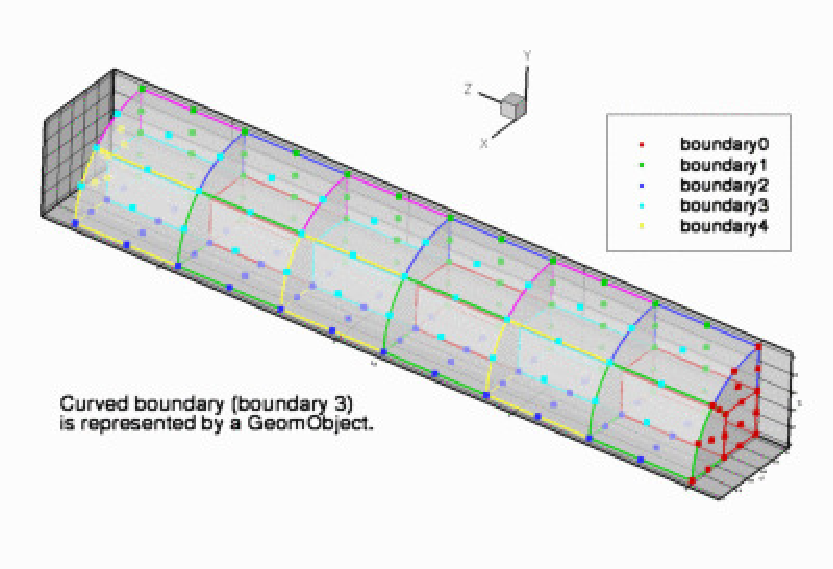
\includegraphics[width=0.75\textwidth]{quarter_tube_mesh}}
\end{DoxyImageNoCaption}
   \\\cline{1-2}
\href{classoomph_1_1TubeMesh.html}{\tt {\bfseries  Tube\+Mesh$<$\+E\+L\+E\+M\+E\+N\+T$>$ }} ~\newline
~\newline

\begin{DoxyItemize}
\item This mesh can be used with all {\ttfamily Finite\+Elements} that are derived from the geometric finite element {\ttfamily Q\+Element$<$3,\+N\+N\+O\+D\+E\+\_\+1\+D$>$}.
\item This mesh forms the basis for numerous derived meshes that describe topologically-\/tube-\/shaped domains.
\item The entire domain is represented by a {\ttfamily Geom\+Object} and the mesh has a {\ttfamily Domain} representation, allowing a {\ttfamily Macro\+Element} -\/ based node update.
\item A refineable version of this mesh exists.
\end{DoxyItemize}{\bfseries Example driver code\+:} ~\newline

\begin{DoxyItemize}
\item The refineable version of this mesh is used in the driver code for \href{../../../navier_stokes/curved_pipe/html/index.html}{\tt the simulation of 3D flow in a curved cylindrical pipe. }
\end{DoxyItemize}& 
\begin{DoxyImageNoCaption}
  \mbox{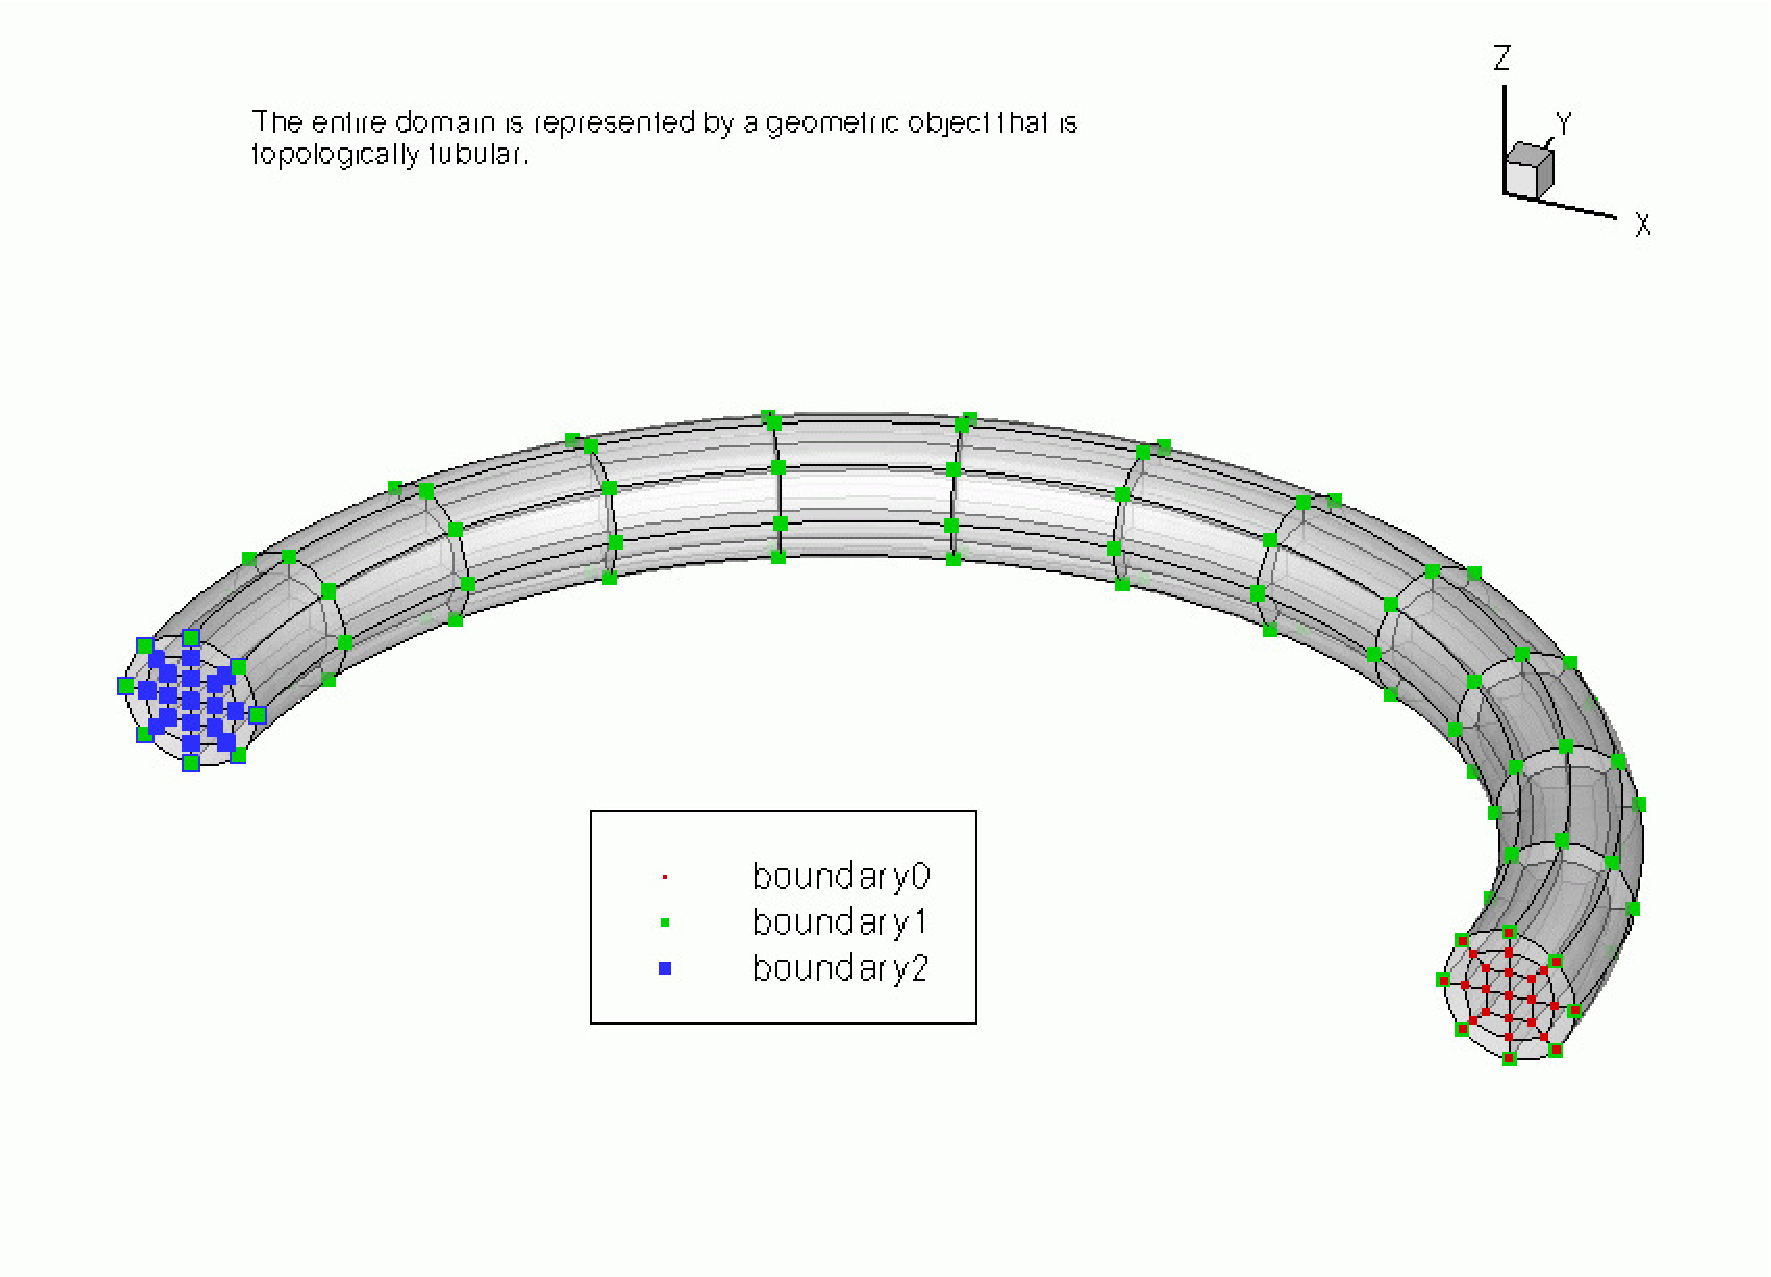
\includegraphics[width=0.75\textwidth]{tube_mesh}}
\end{DoxyImageNoCaption}
   \\\cline{1-2}
\href{classoomph_1_1EighthSphereMesh.html}{\tt {\bfseries  Eighth\+Sphere\+Mesh$<$\+E\+L\+E\+M\+E\+N\+T$>$ }} ~\newline
~\newline

\begin{DoxyItemize}
\item This mesh can be used with all {\ttfamily Finite\+Elements} that are derived from the geometric finite element {\ttfamily Q\+Element$<$3,\+N\+N\+O\+D\+E\+\_\+1\+D$>$}.
\item A refineable version of this mesh exists.
\end{DoxyItemize}{\bfseries Example driver code\+:} ~\newline

\begin{DoxyItemize}
\item The refineable version of this mesh is used in the driver code for \href{../../../poisson/eighth_sphere_poisson/html/index.html}{\tt the adaptive solution of the 3D Poisson equation. }
\end{DoxyItemize}& 
\begin{DoxyImageNoCaption}
  \mbox{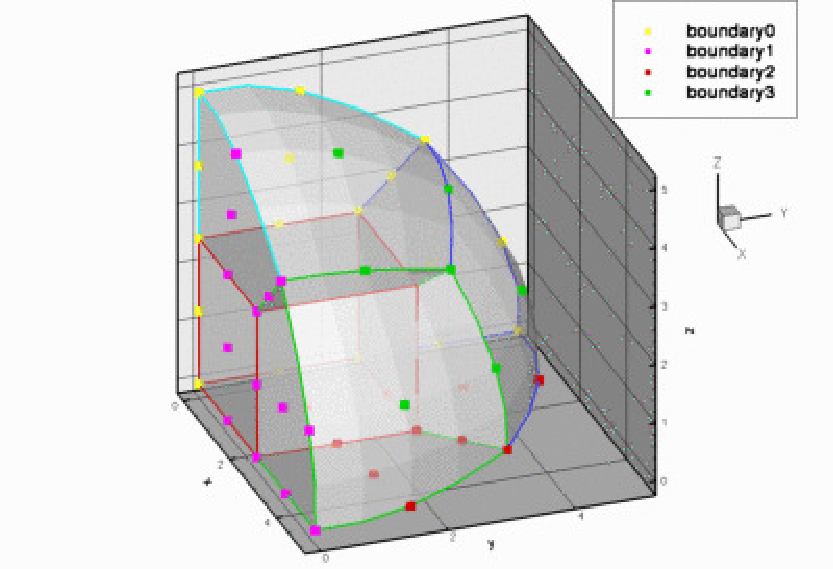
\includegraphics[width=0.75\textwidth]{eighth_sphere_mesh}}
\end{DoxyImageNoCaption}
   \\\cline{1-2}
\end{longtabu}
\end{center} 



 

 \hypertarget{index_pdf}{}\section{P\+D\+F file}\label{index_pdf}
A \href{../latex/refman.pdf}{\tt pdf version} of this document is available. \end{document}
